\documentclass[tikz,border=8pt]{standalone}
% Shared look for every TikZ diagram. Load with \input{../../tools/tikz-style.tex}
\usepackage[T1]{fontenc}
\usepackage{lmodern}
\renewcommand{\sfdefault}{lmr}  % diagrams use the same serif as the text
\usetikzlibrary{arrows.meta, positioning, shapes.geometric, calc, fit, backgrounds}
\definecolor{cblue}{HTML}{4C78A8}
\definecolor{corange}{HTML}{F58518}
\definecolor{cgreen}{HTML}{54A24B}
\definecolor{cred}{HTML}{E45756}
\definecolor{cpurple}{HTML}{B279A2}
\definecolor{cgrey}{HTML}{6B6B6B}
\tikzset{
  every picture/.style={font=\sffamily, line width=1.2pt},
  box/.style={draw=#1, fill=#1!12, rounded corners=4pt, align=center, inner sep=7pt, minimum height=1.1cm},
  box/.default=cgrey,
  arrow/.style={-{Stealth[length=3mm]}, draw=cgrey, line width=1.4pt},
  title/.style={font=\sffamily\bfseries\Large},
  note/.style={font=\sffamily\small, text=cgrey, align=center},
}
\AtBeginDocument{\hyphenpenalty=10000 \exhyphenpenalty=10000}

\begin{document}
\begin{tikzpicture}
  \node[box=cgrey, font=\sffamily\bfseries\large, minimum width=4.6cm] (fs) at (3.5,0) {Feature scaling};
  \node[box=cgrey, fill=white, dashed, font=\sffamily\bfseries, text width=3.6cm, minimum height=1.3cm] (st) at (0.3,-2.1) {Standardization\\[-1pt]\normalfont\small (previous Note)};
  \node[box=cblue, font=\sffamily\bfseries, text width=3.6cm, minimum height=1.3cm] (no) at (6.75,-2.1) {Normalization\\[-1pt]\normalfont\small (this Note)};
  \draw[arrow] (fs.south) -- (st.north);
  \draw[arrow] (fs.south) -- (no.north);
  % the four normalization techniques
  \foreach \name/\col/\f/\r/\use [count=\i] in {
      Min-max scaling/cblue/{$\dfrac{x - x_{\min}}{x_{\max} - x_{\min}}$}/{range 0 to 1}/{known min, max},
      Mean normalization/cgreen/{$\dfrac{x - \bar{x}}{x_{\max} - x_{\min}}$}/{range $-1$ to 1}/{centred data},
      Max-abs scaling/corange/{$\dfrac{x}{|x|_{\max}}$}/{range $-1$ to 1}/{sparse data},
      Robust scaling/cred/{$\dfrac{x - \text{median}}{\text{IQR}}$}/{no fixed range}/{outliers}} {
    \node[box=\col, text width=3.6cm, minimum height=3.6cm, anchor=north] (t\i) at ({0.3 + 4.3*(\i-1)},-4.0)
      {\textbf{\name}\\[6pt] \large \f \\[6pt] \normalsize \r\\[2pt] \small\color{cgrey} use: \use};
    \draw[arrow] (no.south) -- (t\i.north);
  }
\end{tikzpicture}
\end{document}
